\section{CPUs Virtuais}

A classe \textit{VirtualCPU} representa a unidade de básica de processamento de uma \gls{vm}, sendo responsável
pelo encaminhamento de interrupções, pela emulação de exceções e pelo gerenciamento da execução dos \glspl{so} convidados.
Como sua implementação depende da arquitetura da máquina hospedeira, detalhes específicos são apresentados
nas seções correspondentes a cada arquitetura.

\subsection{RISC-V}

O diagrama de classes de \textit{VirtualCPU} - para a arquitetura RISC-V - é ilustrado na Figura~\ref{fig:class-virtual-cpu}.
Para viabilizar a transferência de eventos para a máquina virtual, a classe mantém uma referência direta para a \gls{vm}
à qual está associada. Ademais, esta implementação incorpora o registrador \textit{mtimecmp} emulado para os mecanismos de
temporização, uma vez que existe apenas um registrador físico por máquina hospedeira.
A classe também possui o atributo estático \textit{current\_}, mapeado por núcleo, que armazena um ponteiro para a
instância de \textit{VirtualCPU} em execução em cada núcleo físico.


\vspace{1cm}

\begin{figure}[h]
    \centering
    
\begin{tikzpicture}
        \umlclass[x=0,y=0]{VirtualCPU}{
            - vm\_ : VirtualMachine* \\
            - mtimecmp\_ : uintmax\_t \\
            - sip\_ : uintmax\_t \\
            - current\_ : VirtualCPU*[] \\
        }{
            + VirtualCPU(vm : VirtualMachine*) \\
            + boot\textless Args...\textgreater(args : Args...) : void \\
            + activate() : void \\
            + setInterruptPending() : void \\
            + clearInterruptPending() : void \\
            + onInterProcessorInterrupt() : void \\
            + onTick() : void \\
            + onExternalInterrupt() : void \\
            + mtimecmp() : uintmax\_t \\
            + mtimecmp(value : uintmax\_t) : void \\
            + read(address : uintptr\_t, destination : uintmax\_t*) : bool \\
            + write(address : uintptr\_t, source : uintmax\_t) : bool \\
            + swap(next : VirtualCPU*) : VirtualCPU* \\
            - current() : VirtualCPU* \\
            - current(current : VirtualCPU*) : void \\
            - setTimerInterruptPending() : void \\
            - clearTimerInterruptPending() : void
        }
    \end{tikzpicture}
    \caption{Diagrama de classe da \textit{VirtualCPU}.}
    \label{fig:class-virtual-cpu}
\end{figure}

\subsubsection{Virtualização de Interrupções Temporais}

Interrupções de temporização são virtualizadas por meio do registrador \textit{mtimecmp} emulado em cada instância
de \textit{VirtualCPU}. O \gls{so} convidado atualiza o valor do seu \textit{mtimecmp} por meio de uma \textit{hypercall}.
A partir dessa escrita, e enquanto a respectiva \textit{VirtualCPU} estiver em execução, o hipervisor verifica a cada
\textit{tick} do sistema hospedeiro se o \textit{mtimecmp} do convidado foi atingido ou superado pelo registrador de
tempo global. Caso essa condição seja atendida, uma interrupção é injetada no bit \gls{sti} contido no
\gls{csr} \gls{sip} do convidado.

\subsubsection{Virtualização de Interrupções Externas}

Interrupções externas não são controladas diretamente pela \textit{VirtualCPU}; tal classe fica responsável apenas por
injetá-las no sistema convidado. Para isso, a \textit{VirtualCPU} expõe uma interface para que outros dispositivos sejam
capazes de gerar esses eventos. Tais eventos são injetados por meio da sinalização do bit \gls{sei} no \gls{csr} \gls{sip}
do convidado.

\subsubsection{Inicialização}

A inicialização de uma \textit{VirtualCPU} RISC-V consiste na preparação do ambiente de execução e na subsequente
transição para o ponto de entrada da \gls{vm} já em modo supervisor; uma vez que a maioria dos \glspl{so} convidados -
como o Linux - esperam inicializar nesse modo.

O fluxo ordenado das etapas executadas durante esse processo de inicialização está ilustrado na
Figura~\ref{fig:class-virtual-cpu-boot}:

\vspace{1cm}

\begin{figure}[H]
	\begin{center}
	    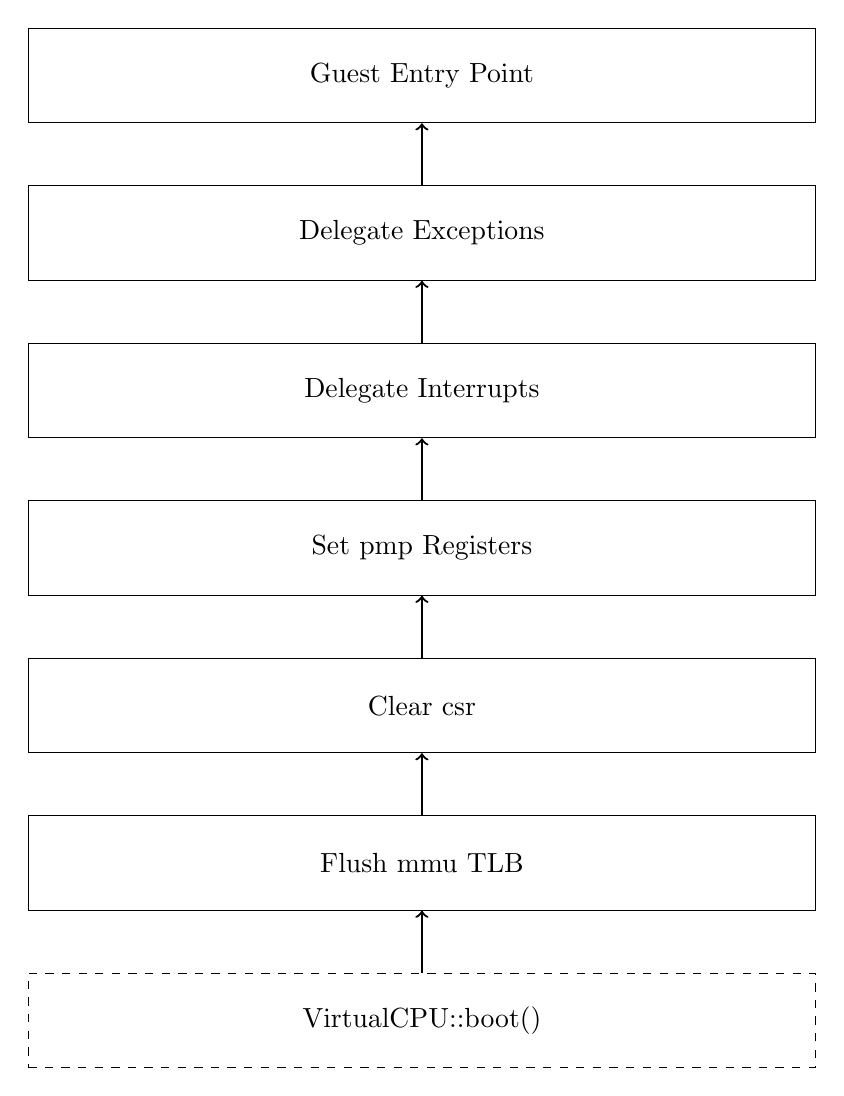
\begin{tikzpicture}
	        \node[rectangle, minimum width=10cm, minimum height=1.2cm, draw, align=center, dashed] (A) at (0,2){VirtualCPU::boot()};
			\node[rectangle, minimum width=10cm, minimum height=1.2cm, draw, align=center] (B) at (0,4){Flush \gls{mmu} TLB};
			\node[rectangle, minimum width=10cm, minimum height=1.2cm, draw, align=center] (C) at (0,6){Clear \glspl{csr}};
			\node[rectangle, minimum width=10cm, minimum height=1.2cm, draw, align=center] (D) at (0,8){Set \gls{pmp} Registers};
	        \node[rectangle, minimum width=10cm, minimum height=1.2cm, draw, align=center] (E) at (0,10){Delegate Interrupts};
	        \node[rectangle, minimum width=10cm, minimum height=1.2cm, draw, align=center] (F) at (0,12){Delegate Exceptions};
	        \node[rectangle, minimum width=10cm, minimum height=1.2cm, draw, align=center] (G) at (0,14){Guest Entry Point};
	        \draw[->, thick] (A) -- (B);
	        \draw[->, thick] (B) -- (C);
	        \draw[->, thick] (C) -- (D);
	        \draw[->, thick] (D) -- (E);
			\draw[->, thick] (E) -- (F);
			\draw[->, thick] (F) -- (G);
	    \end{tikzpicture}
	\end{center}
	\caption{Fluxo Geral de Inicialização de uma \textit{VirtualCPU} RISC-V.}
    \label{fig:class-virtual-cpu-boot}
\end{figure}
